\documentclass[a4paper,12pt]{article}
\usepackage{iftex}
\ifPDFTeX
  \usepackage[utf8]{vietnam}
\else
  \usepackage{fontspec}
  \usepackage[vietnamese]{babel}
\fi
\usepackage{a4wide,amssymb,latexsym,multicol,array,hhline,fancyhdr}
\usepackage{booktabs}
\usepackage{amsmath}
\usepackage{lastpage}
\usepackage{enumerate}
\usepackage{color}
\usepackage{graphicx}
\usepackage{float}
\usepackage{tabularx, caption}
\usepackage{multirow}
\usepackage[framemethod=tikz]{mdframed}
\usepackage{geometry}
\usepackage{setspace}
\usepackage{tikz}
\usepackage{listings}
\usepackage{hyperref}

\geometry{
  a4paper,
  top=25mm,
  bottom=25mm,
  left=30mm,
  right=20mm
}

\hypersetup{
  urlcolor=blue,
  linkcolor=black,
  citecolor=black,
  colorlinks=true
}

\setlength{\headheight}{40pt}
\pagestyle{fancy}
\fancyhead{}
\fancyhead[L]{
  \begin{tabular}{rl}
    \begin{picture}(25,15)(0,0)
      \put(0,-8){
\includegraphics[width=8mm, height=8mm]{logoITSGUsmall.png}}
    \end{picture}&
    \begin{tabular}{l}
      \textbf{\ttfamily Trường Đại học Sài Gòn}\\
      \textbf{\ttfamily Khoa Công Nghệ Thông Tin}
    \end{tabular}
  \end{tabular}
}
\fancyhead[R]{
  \begin{tabular}{r}
    \tiny \bf CÔNG NGHỆ PHẦN MỀM \\
    \tiny \bf ASSIGNMENT 1 -- BREWLITE
  \end{tabular}
}
\fancyfoot{}
\fancyfoot[L]{\scriptsize \ttfamily Bài tập lớn môn Công nghệ Phần mềm -- Học kỳ I Năm học 2026--2027}
\fancyfoot[R]{\scriptsize \ttfamily Trang {\thepage}/\pageref{LastPage}}
\renewcommand{\headrulewidth}{0.3pt}
\renewcommand{\footrulewidth}{0.3pt}

\setcounter{secnumdepth}{4}
\setcounter{tocdepth}{3}

\definecolor{dkgreen}{rgb}{0,0.6,0}
\definecolor{gray}{rgb}{0.5,0.5,0.5}
\definecolor{mauve}{rgb}{0.58,0,0.82}
\definecolor{codebg}{rgb}{0.96,0.96,0.96}

\lstset{
  backgroundcolor=\color{codebg},
  basicstyle=\small\ttfamily,
  breaklines=true,
  breakatwhitespace=true,
  frame=single,
  numbers=left,
  numbersep=5pt,
  numberstyle=\tiny\color{gray},
  keywordstyle=\color{blue},
  commentstyle=\color{dkgreen},
  stringstyle=\color{mauve},
  tabsize=2,
  showstringspaces=false
}

\begin{document}

\begin{titlepage}
\begin{center}
  \textbf{\large TRƯỜNG ĐẠI HỌC SÀI GÒN} \\
  \textbf{\large KHOA CÔNG NGHỆ THÔNG TIN} \\
  \vspace{0.8cm}
  
\includegraphics[width=3.2cm]{logoITSGU.png} \\
  \vspace{1cm}

  \textbf{\Large BÁO CÁO BÀI TẬP LỚN -- ASSIGNMENT 1} \\[0.3cm]
  \textbf{\Huge MÔN CÔNG NGHỆ PHẦN MỀM} \\[0.5cm]
  \rule{\textwidth}{0.6pt} \\[0.4cm]
  \textbf{\Large ĐỀ TÀI: BREWLITE} \\[0.2cm]
  \textbf{\LARGE ỨNG DỤNG ĐẶT CÀ PHÊ KHÔNG DÙNG TIỀN MẶT} \\[0.2cm]
  \textbf{\LARGE THEO QUY TRÌNH AGILE SCRUM (10 TASKS)} \\[0.3cm]
  \textit{\large (Product Vision, Scrum Backlog, MVP End-to-End \& Backend Concurrency)} \\[0.4cm]
  \rule{\textwidth}{0.6pt}
\end{center}

\vspace{1.5cm}

\begin{table}[h!]
\centering
\begin{tabular}{rrl}
  \textbf{Giảng viên hướng dẫn:} & & \textbf{ThS. Từ Lãng Phiêu} \\
  \vspace{0.2cm} \\
  \textbf{Sinh viên thực hiện:}   & & Nguyễn Tấn Phát -- MSSV: 3124410265 \\
  \vspace{0.2cm} \\
  \textbf{Lớp:}                   & & DCT1243 \\
  \textbf{Khoá học:}              & & 2024 -- 2028
\end{tabular}
\end{table}

\vfill

\begin{center}
  \textbf{TP. HỒ CHÍ MINH, NĂM 2026}
\end{center}
\end{titlepage}

\thispagestyle{empty}
\newpage

\tableofcontents
\newpage

\section{Tổng quan sản phẩm và Quy trình Agile Scrum}

\subsection{Tầm nhìn sản phẩm (Product Vision) và Các bên liên quan}
\textbf{Product Vision:} \textit{``BrewLite giúp khách hàng đặt và thanh toán đồ uống không dùng tiền mặt chỉ trong vài chạm, giảm thời gian xếp hàng và nhận đơn nhanh tại quầy.''}

Hệ thống xác định 6 nhóm bên liên quan (Stakeholders) theo đặc tả gốc Assignment 1:
\begin{enumerate}[1.]
  \item \textbf{Khách hàng (Customer / Member):} Duyệt thực đơn, chọn kích cỡ (Size S/M/L) và topping, áp mã khuyến mãi, thanh toán không dùng tiền mặt và theo dõi trạng thái đơn hàng.
  \item \textbf{Nhân viên quầy (Barista):} Tiếp nhận đơn đã thanh toán (\texttt{PAID}) và cập nhật tiến độ pha chế (\texttt{PREPARING} $\rightarrow$ \texttt{READY} $\rightarrow$ \texttt{COMPLETED}).
  \item \textbf{Quản lý cửa hàng / Product Owner:} Xác định yêu cầu nghiệp vụ, sắp xếp ưu tiên Product Backlog và nghiệm thu Increment sau mỗi Sprint.
  \item \textbf{Giảng viên nghiệm thu:} Đánh giá quy trình Agile Scrum, tính đầy đủ của 10 Tasks và chất lượng kỹ thuật sản phẩm bàn giao.
  \item \textbf{Sinh viên thực hiện (Development Team):} Phân tích yêu cầu, thiết kế, hiện thực Frontend/Backend, viết kiểm thử tự động và vận hành đóng gói bàn giao.
  \item \textbf{Đơn vị thanh toán (Payment Gateway):} Cổng thanh toán mô phỏng Ví điện tử (MoMo/VNPay/Ví BrewLite) và Thẻ ngân hàng phục vụ kiểm thử luồng thành công, thất bại và chống lặp giao dịch.
\end{enumerate}

\subsection{Áp dụng quy trình Agile Scrum}
Dự án áp dụng đầy đủ các thành phần cốt lõi của Agile Scrum:
\begin{itemize}
  \item \textbf{Tạo phẩm (Artifacts):} Product Backlog quản lý toàn bộ 10 Tasks (\texttt{docs/sprint/product-backlog.md}), Sprint Backlog cho từng vòng lặp (\texttt{sprint-1-backlog.md}, \texttt{sprint-2-backlog.md}) và Increment chạy được sau mỗi Sprint.
  \item \textbf{Sự kiện (Events):} Sprint Planning, cập nhật tiến độ hằng ngày theo biểu đồ Burndown, Sprint Review nghiệm thu luồng End-to-End và Sprint Retrospective rút kinh nghiệm cải tiến.
  \item \textbf{Phân bổ Sprint thực tế:}
    \begin{itemize}
      \item \textbf{Sprint 1 (23 / 23 SP):} Hoàn thành nền tảng dự án, Products API, Database Seed và giao diện Menu + Tùy biến Size/Topping (Tasks 1, 2, 3, 4).
      \item \textbf{Sprint 2 (33 / 33 SP):} Hoàn thành Giỏ hàng Zustand, API tạo đơn, xác thực JWT, thanh toán không tiền mặt, lịch sử đơn, Docker Compose 3 services và toàn bộ nghiệp vụ Backend nâng cao (Tasks 5, 6, 7, 8, 9, 10).
    \end{itemize}
\end{itemize}

\subsection{Biểu đồ theo dõi tiến độ (Sprint 2 Burndown Chart)}
Tổng cam kết Sprint 2 là \textbf{33 Story Points} trong 10 ngày làm việc (tốc độ lý tưởng $3.3$ SP/ngày). Khối lượng công việc còn lại được cập nhật cuối mỗi ngày làm việc như bảng dưới đây:

\begin{table}[h!]
\centering
\scriptsize
\begin{tabular}{|l|c|c|c|c|c|c|c|c|c|c|c|}
\hline
\textbf{Ngày làm việc} & \textbf{D0} & \textbf{D1} & \textbf{D2} & \textbf{D3} & \textbf{D4} & \textbf{D5} & \textbf{D6} & \textbf{D7} & \textbf{D8} & \textbf{D9} & \textbf{D10} \\
\hline
\textbf{Lý tưởng (Ideal SP)} & 33.0 & 29.7 & 26.4 & 23.1 & 19.8 & 16.5 & 13.2 & 9.9 & 6.6 & 3.3 & 0.0 \\
\hline
\textbf{Thực tế (Actual SP)} & 33 & 30 & 25 & 23 & 20 & 17 & 12 & 10 & 8 & 3 & 0 \\
\hline
\end{tabular}
\caption{Nhật ký theo dõi Burndown Chart Sprint 2 (Hoàn thành 33/33 SP -- 100\%)}
\end{table}

\newpage
\section{Yêu cầu phần mềm, Luồng nghiệp vụ và Kiến trúc MVP}

\subsection{Yêu cầu chức năng, Phi chức năng và Danh mục User Stories}
\begin{itemize}
  \item \textbf{Yêu cầu chức năng (6 nhóm cốt lõi):} (1) Hiển thị thực đơn kèm ảnh, tên, giá định dạng VND và bộ lọc danh mục; (2) Xem chi tiết sản phẩm, chọn Size (S/M/L) và đa Topping; (3) Quản lý giỏ hàng (thêm/sửa/xóa, tự tính tổng tiền, lưu bền vững); (4) Đăng ký/Đăng nhập bằng JWT; (5) Tạo đơn hàng và thanh toán không dùng tiền mặt; (6) Hiển thị màn hình xác nhận (mã đơn \texttt{\#xxxxxx}, trạng thái \texttt{PAID}) và lịch sử đơn hàng.
  \item \textbf{Yêu cầu phi chức năng:} Thời gian phản hồi API dưới $500$ms (đo thực tế trên AWS EC2 đạt độ trễ CSDL $1$ms); mật khẩu băm bằng \texttt{bcrypt} (salt $\ge 10$), bảo vệ endpoint bằng \texttt{JwtAuthGuard}, kiểm tra dữ liệu đầu vào bằng \texttt{ValidationPipe}; giao diện Mobile-First tương thích tốt trên di động và máy tính.
\end{itemize}

\begin{table}[h!]
\centering
\scriptsize
\begin{tabularx}{\textwidth}{|c|l|X|}
\hline
\textbf{Mã US} & \textbf{Vai trò} & \textbf{Đặc tả User Story (Tài liệu chi tiết: \texttt{docs/requirements/user-stories.md})} \\
\hline
\textbf{US-01} & Lập trình viên & Là một lập trình viên, tôi muốn khởi tạo Monorepo (\texttt{frontend/}, \texttt{backend/}, \texttt{docs/}), Git và \texttt{README.md}, để cả hệ thống có nền tảng thống nhất dễ chạy và kiểm thử. \\
\hline
\textbf{US-02} & Khách hàng & Là một khách hàng, tôi muốn hệ thống có API \texttt{GET /products} lấy thực đơn từ PostgreSQL kèm danh mục và topping, để luôn xem được món đang phục vụ và giá chính xác. \\
\hline
\textbf{US-03} & Khách hàng & Là một khách hàng, tôi muốn duyệt thực đơn theo Tabs danh mục, tìm kiếm món và thấy trạng thái tải/rỗng/lỗi rõ ràng trên di động, để chọn nước nhanh chóng. \\
\hline
\textbf{US-04} & Khách hàng & Là một khách hàng, tôi muốn mở chi tiết món để chọn Size (S/M/L), đa Topping, nhập ghi chú và xem giá cập nhật tức thì, để đặt đúng ly nước theo sở thích. \\
\hline
\textbf{US-05} & Khách hàng & Là một khách hàng, tôi muốn thêm/sửa/xóa món trong giỏ hàng và lưu bền vững qua \texttt{localStorage}, để không mất đơn khi tải lại trang hoặc đăng nhập. \\
\hline
\textbf{US-06} & Khách hàng & Là một khách hàng, tôi muốn tạo đơn hàng trạng thái \texttt{PENDING} với tổng tiền tính lại hoàn toàn trên Server, để đảm bảo minh bạch và chống gian lận giá. \\
\hline
\textbf{US-07} & Thành viên & Là một khách hàng, tôi muốn đăng ký và đăng nhập bảo mật bằng JWT, để bảo vệ thông tin cá nhân, lịch sử đơn và điểm thưởng của riêng tôi. \\
\hline
\textbf{US-08} & Khách hàng & Là một khách hàng, tôi muốn thanh toán không dùng tiền mặt (Ví/Thẻ mô phỏng hoặc VietQR PayOS thật) và giữ giỏ hàng nếu lỗi, để trả tiền nhanh không cần tiền mặt. \\
\hline
\textbf{US-09} & Khách hàng & Là một khách hàng, tôi muốn thấy màn hình xác nhận kèm mã đơn \texttt{\#xxxxxx} và tra cứu lịch sử (\texttt{GET /orders/me}), để theo dõi đơn tại quầy. \\
\hline
\textbf{US-10} & Thành viên & Là một khách thành viên, tôi muốn đơn hàng tuân thủ State Machine, chống trừ tiền 2 lần (\texttt{Idempotency-Key}), chống vượt tồn kho (\texttt{Optimistic Lock}), áp Voucher và cộng điểm Loyalty, để giao dịch an toàn tuyệt đối. \\
\hline
\end{tabularx}
\caption{Danh mục 10 User Stories cốt lõi của hệ thống BrewLite (Assignment 1)}
\end{table}

\subsection{Luồng nghiệp vụ từ chọn sản phẩm đến thanh toán}
Luồng nghiệp vụ chính (Happy Path) của BrewLite MVP:
$$\text{Mở app} \rightarrow \text{Xem menu} \rightarrow \text{Chọn Size/Topping} \rightarrow \text{Giỏ hàng} \rightarrow \text{Đăng nhập JWT} \rightarrow \text{Thanh toán} \rightarrow \text{Xác nhận đơn}$$
Khi thanh toán gặp lỗi, đơn chuyển sang trạng thái \texttt{PAYMENT\_FAILED}, giỏ hàng được giữ nguyên để khách hàng thử lại mà không cần chọn lại từ đầu.

\begin{figure}[H]
  \centering
  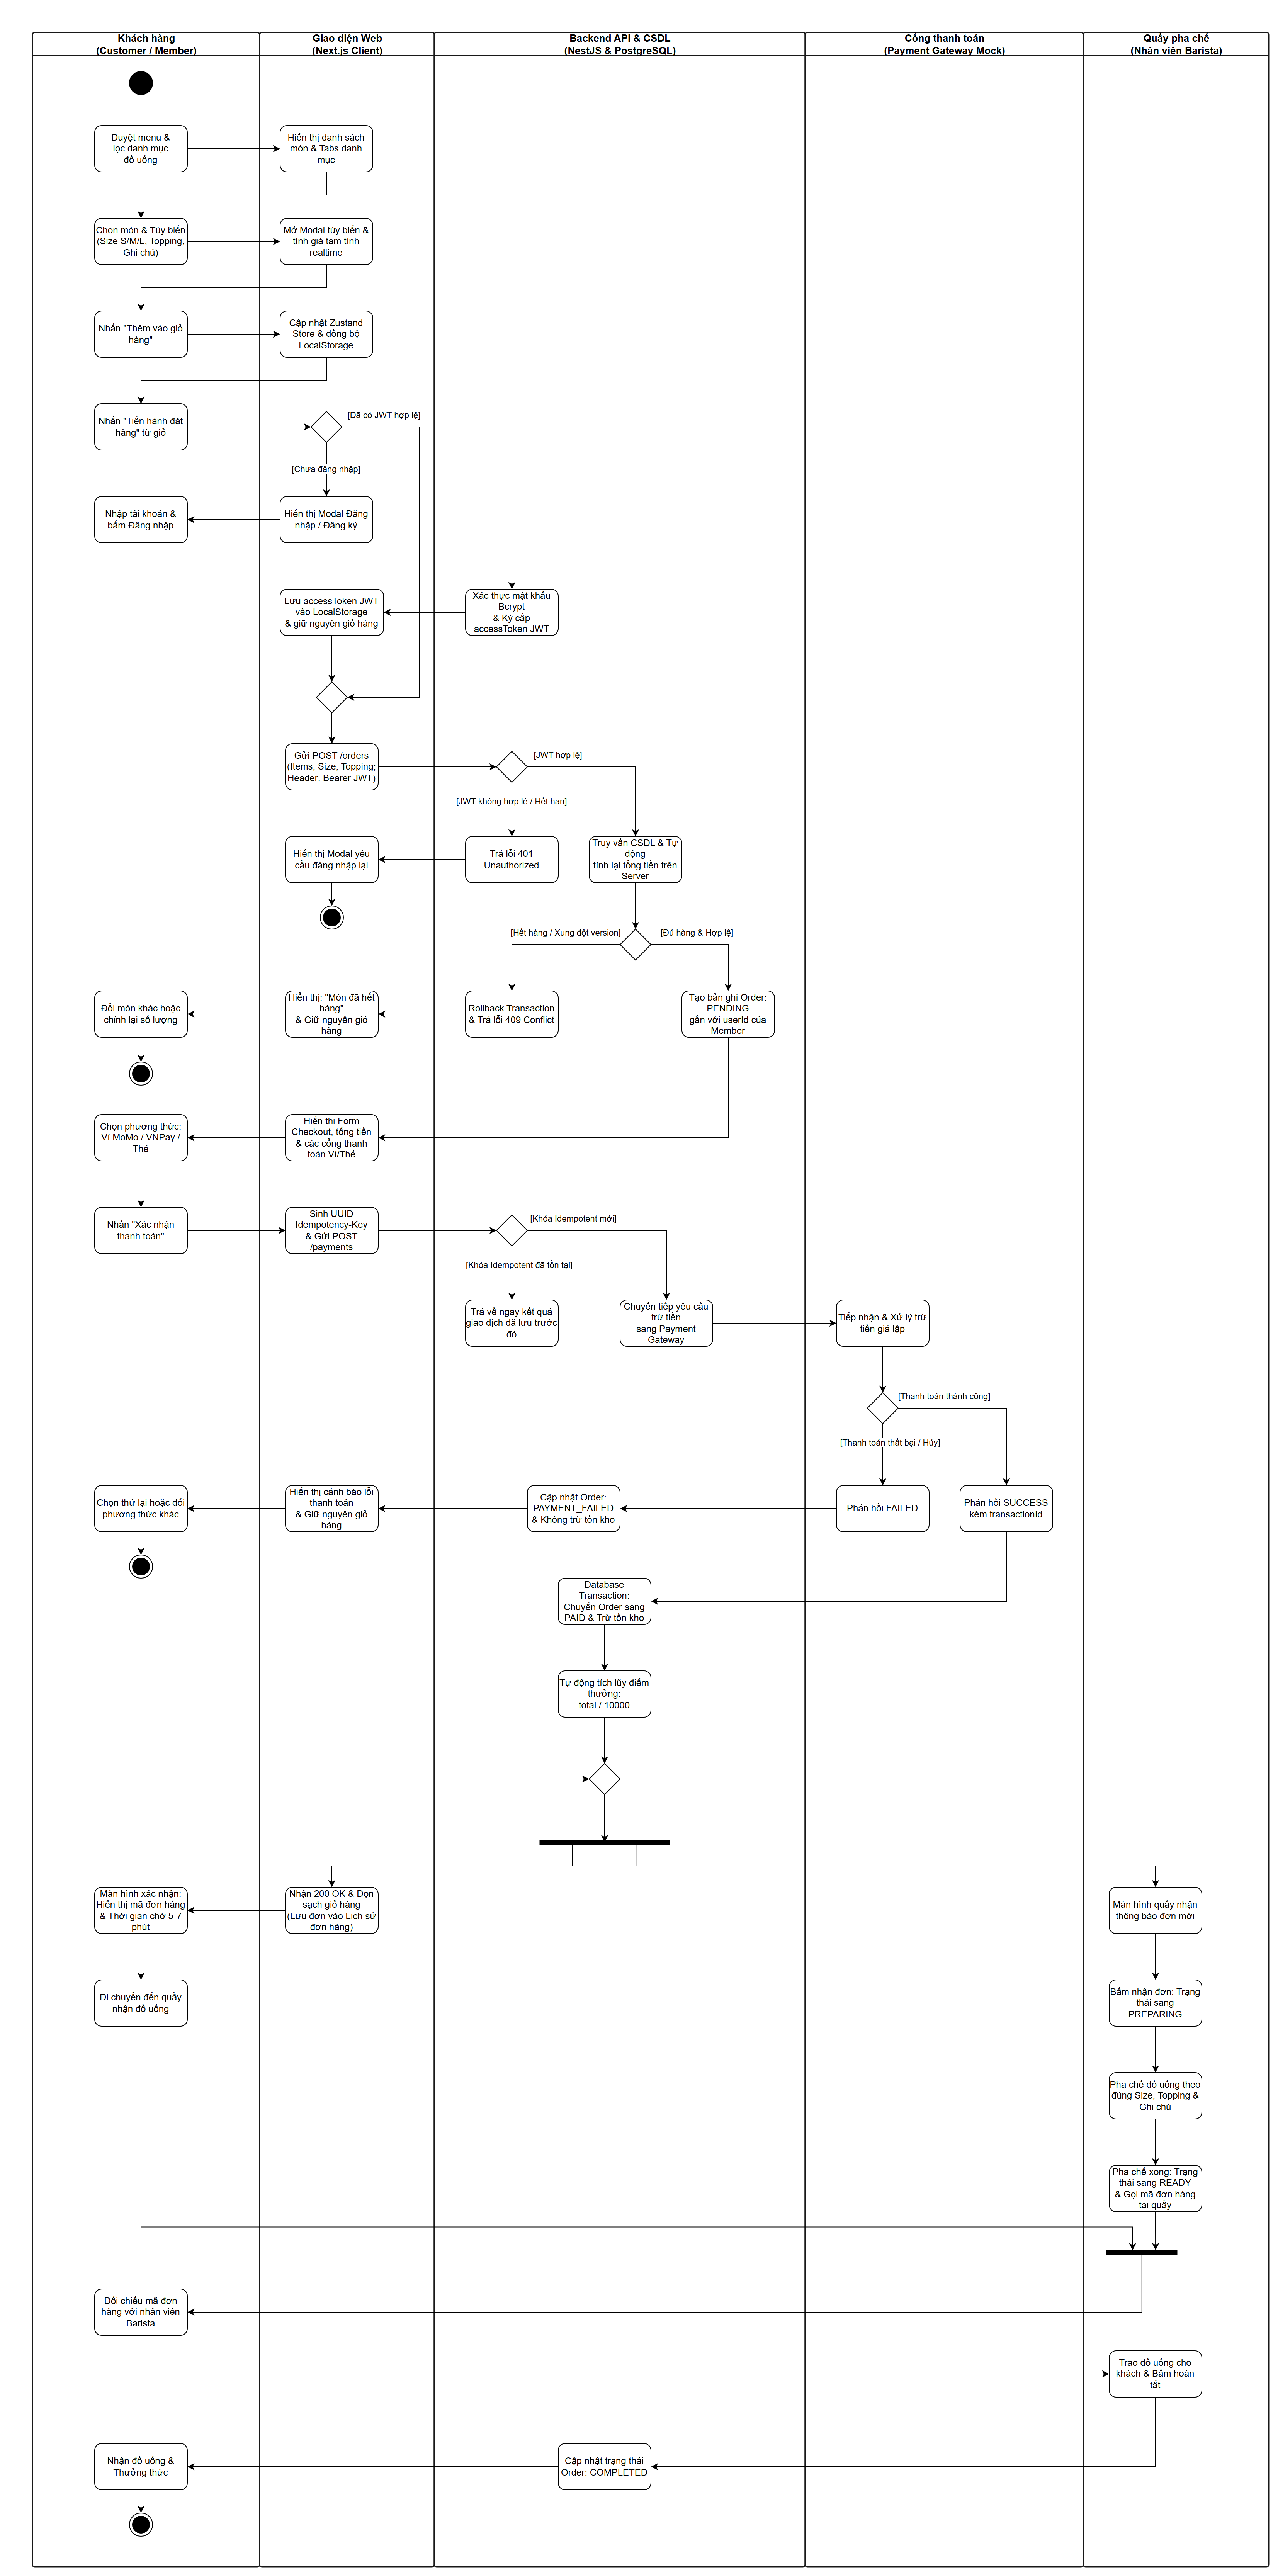
\includegraphics[width=\textwidth,height=0.72\textheight,keepaspectratio]{figures/activity-flow.png}
  \caption{Sơ đồ hoạt động luồng nghiệp vụ gọi món và thanh toán BrewLite}
  \label{fig:a1-activity}
\end{figure}

\subsection{Kiến trúc công nghệ và 5 màn hình MVP cốt lõi}
\begin{table}[h!]
\centering
\small
\begin{tabularx}{\textwidth}{|l|X|}
\hline
\textbf{Thành phần} & \textbf{Công nghệ hiện thực trong dự án} \\
\hline
\textbf{Frontend} & Next.js 16.3.5 (App Router, React 19, TypeScript), Tailwind CSS v4, Zustand (\texttt{useCartStore}, \texttt{useAuthStore} lưu \texttt{localStorage}). \\
\hline
\textbf{Backend} & NestJS 10.4 (TypeScript), REST API theo kiến trúc Modular Monolith, \texttt{class-validator}, Passport JWT, \texttt{bcrypt}. \\
\hline
\textbf{Cơ sở dữ liệu} & PostgreSQL 16 + Prisma ORM 6.19 (Migrations có phiên bản + Database Seed tự động). \\
\hline
\textbf{Thanh toán} & \texttt{PaymentsService} mô phỏng Ví điện tử (MoMo/VNPay/Ví BrewLite) và Thẻ ngân hàng kèm cơ chế \texttt{Idempotency-Key}. \\
\hline
\textbf{DevOps \& Bàn giao} & Docker Multi-stage, \texttt{docker-compose.yml} (3 services), GitHub Actions CI/CD, AWS EC2 Ubuntu + Nginx SSL HTTPS. \\
\hline
\end{tabularx}
\caption{Bảng ngăn xếp công nghệ hiện thực BrewLite MVP}
\end{table}

Năm màn hình cốt lõi theo đặc tả wireframe Mục 7 Assignment 1 đã được hiện thực đầy đủ: (1) Trang \textbf{Menu} (\texttt{page.tsx}, \texttt{CategoryFilter}, \texttt{ProductCard}); (2) Modal \textbf{Chi tiết món} (\texttt{ProductDetailModal}); (3) Ngăn kéo \textbf{Giỏ hàng} (\texttt{CartDrawer}); (4) Modal \textbf{Thanh toán} (\texttt{CheckoutModal}); và (5) Modal \textbf{Xác nhận đơn} (\texttt{OrderConfirmationModal}) kèm \textbf{Lịch sử đơn hàng} (\texttt{OrderHistoryModal}).

\newpage
\section{Product Backlog và Hiện thực 10 Tasks theo Scrum}

Toàn bộ 10/10 Tasks (tổng 10 điểm theo thang điểm Assignment 1) đã hoàn thành 100\%, vượt qua toàn bộ bộ kiểm thử tự động và đạt chuẩn Definition of Done:

\begin{table}[h!]
\centering
\scriptsize
\begin{tabularx}{\textwidth}{|c|l|X|c|}
\hline
\textbf{\#} & \textbf{Tên Task (Story)} & \textbf{Thành phần hiện thực thực tế trong mã nguồn} & \textbf{Trạng thái} \\
\hline
\textbf{1} & Khởi tạo dự án \& cấu trúc & Monorepo gồm \texttt{frontend/} (Next.js 16), \texttt{backend/} (NestJS 10), \texttt{docs/}, \texttt{.env.example}, \texttt{README.md}, Git Conventional Commits. & 1/1 (Done) \\
\hline
\textbf{2} & API danh sách sản phẩm & \texttt{ProductsModule}: \texttt{GET /products}, \texttt{GET /products/:id}, \texttt{GET /products/categories}, \texttt{GET /products/toppings} + \texttt{prisma/seed.ts} (12 món, 4 danh mục, 6 topping). & 1/1 (Done) \\
\hline
\textbf{3} & Trang Menu (Frontend) & \texttt{page.tsx}, \texttt{CategoryFilter.tsx}, \texttt{ProductCard.tsx}; lọc danh mục, tìm kiếm, hiển thị đủ 3 trạng thái Skeleton, Empty, Error. & 1/1 (Done) \\
\hline
\textbf{4} & Chi tiết \& Tùy chọn món & \texttt{ProductDetailModal.tsx}: chọn Size (S/M/L), đa Topping, ghi chú cho Barista, tính tổng giá realtime và hỗ trợ bàn phím ARIA. & 1/1 (Done) \\
\hline
\textbf{5} & Giỏ hàng (Cart) & \texttt{useCartStore.ts} (Zustand + \texttt{localStorage}), \texttt{CartDrawer.tsx}, đồng bộ badge số lượng trên \texttt{Header.tsx}, gộp món trùng tùy biến. & 1/1 (Done) \\
\hline
\textbf{6} & API tạo đơn hàng & \texttt{OrdersModule}: \texttt{POST /orders} validate bằng \texttt{class-validator}, tính lại giá hoàn toàn phía Server từ CSDL, lưu đơn trạng thái \texttt{PENDING}. & 1/1 (Done) \\
\hline
\textbf{7} & Đăng ký / Đăng nhập JWT & \texttt{AuthModule}: \texttt{POST /auth/register}, \texttt{POST /auth/login}, \texttt{GET /auth/me}; băm mật khẩu \texttt{bcrypt}; \texttt{JwtAuthGuard} bảo vệ toàn bộ route đơn hàng \& thanh toán. & 1/1 (Done) \\
\hline
\textbf{8} & Thanh toán không tiền mặt & \texttt{PaymentsModule}: \texttt{POST /payments} + \texttt{CheckoutModal.tsx}; chọn Ví/Thẻ; thành công chuyển \texttt{PAID}, thất bại chuyển \texttt{PAYMENT\_FAILED} và giữ nguyên giỏ hàng. & 1/1 (Done) \\
\hline
\textbf{9} & Xác nhận, Lịch sử \& Bàn giao & \texttt{OrderConfirmationModal.tsx} (mã \texttt{\#xxxxxx}), \texttt{OrderHistoryModal.tsx} (\texttt{GET /orders/me}), \texttt{docker-compose.yml} 3 services, \texttt{README.md}, demo live HTTPS. & 1/1 (Done) \\
\hline
\textbf{10} & Nghiệp vụ Backend nâng cao & Order State Machine (\texttt{assertTransition}), thanh toán Idempotent (\texttt{Idempotency-Key}), Optimistic Locking (\texttt{version}), Voucher \& Loyalty kèm bộ test chứng minh \texttt{(a)(b)(c)}. & 1/1 (Done) \\
\hline
\end{tabularx}
\caption{Bảng tổng hợp nghiệm thu 10 Tasks trong Product Backlog (Assignment 1)}
\end{table}

\newpage
\section{Chuyên sâu Task 10 -- Nghiệp vụ Backend và Kiểm thử chứng minh}

\subsection{Máy trạng thái đơn hàng (Order State Machine)}
Tệp \texttt{backend/src/orders/order-state-machine.ts} hiện thực ma trận chuyển tiếp hợp lệ $7 \times 7$ thông qua hàm \texttt{assertTransition(currentStatus, nextStatus)}:
\begin{itemize}
  \item \textbf{Luồng thành công chính:} \texttt{PENDING} $\rightarrow$ \texttt{PAID} $\rightarrow$ \texttt{PREPARING} $\rightarrow$ \texttt{READY} $\rightarrow$ \texttt{COMPLETED}.
  \item \textbf{Các nhánh ngoại lệ hợp lệ:}
    \begin{itemize}
      \item Thanh toán lỗi và thử lại: \texttt{PENDING} $\rightarrow$ \texttt{PAYMENT\_FAILED} $\rightarrow$ \texttt{PENDING}.
      \item Hủy đơn hàng: \texttt{PENDING} $\rightarrow$ \texttt{CANCELLED}, \texttt{PAYMENT\_FAILED} $\rightarrow$ \texttt{CANCELLED}, và \texttt{PAID} $\rightarrow$ \texttt{CANCELLED} (tự động hoàn lại tồn kho sản phẩm trong cùng giao dịch).
    \end{itemize}
  \item \textbf{Chặn chuyển trạng thái sai:} \texttt{COMPLETED} và \texttt{CANCELLED} là hai trạng thái kết thúc; mọi hành vi nhảy cóc (ví dụ \texttt{PENDING} $\rightarrow$ \texttt{READY} hoặc \texttt{COMPLETED} $\rightarrow$ \texttt{PAID}) bị chặn ngay lập tức với ngoại lệ HTTP \texttt{400 Bad Request}.
\end{itemize}

\subsection{Thanh toán Idempotent (Chống trừ tiền trùng lặp)}
Endpoint \texttt{POST /payments} bắt buộc header \texttt{Idempotency-Key} (UUIDv4 sinh ở Client cho mỗi phiên thanh toán) và ràng buộc duy nhất (\texttt{@unique}) trên cột \texttt{Payment.idempotencyKey}:
\begin{itemize}
  \item Khi nhận request có \texttt{Idempotency-Key} đã tồn tại, \texttt{PaymentsService} trả về trực tiếp kết quả giao dịch đã ghi nhận trước đó mà không trừ tiền, không trừ tồn kho và không cộng điểm thưởng lần thứ hai.
  \item Nếu cùng một đơn hàng nhận hai yêu cầu đồng thời với hai khóa khác nhau (double-tab), giao dịch thứ hai bị từ chối với HTTP \texttt{409 Conflict}.
\end{itemize}

\subsection{Kiểm soát tồn kho đồng thời (Transaction + Optimistic Locking)}
Bảng \texttt{Product} bổ sung trường số nguyên \texttt{version Int @default(1)}. Trong cùng một giao dịch ACID (\texttt{prisma.\$transaction}) khi xác nhận thanh toán thành công:
\begin{itemize}
  \item Hệ thống cập nhật tồn kho bằng lệnh điều kiện nguyên tử: \texttt{WHERE id = :id AND version = :expectedVersion AND stock >= :qty}, đồng thời tăng \texttt{version = version + 1}.
  \item Nếu có giao dịch đồng thời làm thay đổi \texttt{version} hoặc tồn kho không đủ, số bản ghi cập nhật trả về \texttt{0}, giao dịch tự động Rollback toàn bộ và ném lỗi HTTP \texttt{409 Conflict}, ngăn chặn tuyệt đối bán âm tồn kho (overselling).
\end{itemize}

\subsection{Khuyến mãi Voucher và Tích điểm thành viên (Loyalty)}
\begin{itemize}
  \item \textbf{Voucher:} Endpoint \texttt{GET /vouchers/validate} kiểm tra mã khuyến mãi hợp lệ (\texttt{BREWLITEFIRST} giảm 20\%, \texttt{COFFEELOVER} giảm 15\%), kiểm tra hạn dùng và mức chiết khấu tối đa; số tiền giảm được tính lại hoàn toàn ở Backend khi gọi \texttt{POST /orders}.
  \item \textbf{Điểm thưởng Loyalty:} Ngay khi đơn chuyển sang trạng thái \texttt{PAID} trong \texttt{prisma.\$transaction}, hệ thống cộng thêm \texttt{Math.floor(finalAmount / 10000)} điểm vào \texttt{User.loyaltyPoints} và hiển thị ngay trên \texttt{OrderConfirmationModal} và \texttt{Header}.
\end{itemize}

\subsection{Bằng chứng kiểm thử tự động cho 3 tiêu chí (a), (b), (c)}
Toàn bộ dự án sở hữu \textbf{32 test suites / 143 test cases} (Backend Unit/Integration: \textbf{17 suites / 89 tests}; Backend Supertest HTTP E2E: \textbf{1 suite / 1 full-flow test}; Frontend Component/Store/Page: \textbf{14 suites / 53 tests}) đều vượt qua 100\%. Bảng dưới đây đối chiếu trực tiếp 3 tiêu chí chấm bắt buộc của Task 10:

\begin{table}[h!]
\centering
\scriptsize
\begin{tabularx}{\textwidth}{|c|X|l|c|}
\hline
\textbf{Tiêu chí} & \textbf{Kịch bản kiểm thử tự động đã chứng minh} & \textbf{Tệp kiểm thử} & \textbf{Kết quả} \\
\hline
\textbf{(a)} & Kiểm thử trọn vẹn 49 cặp chuyển trạng thái ($7 \times 7$) của \texttt{assertTransition}, xác nhận chặn 100\% chuyển tiếp nhảy cóc/sai quy tắc bằng \texttt{BadRequestException}. & \texttt{order-state-machine.spec.ts} & \textbf{PASS} \\
\hline
\textbf{(b)} & Gửi đồng thời 5 request \texttt{POST /payments} cùng \texttt{Idempotency-Key}: chỉ tạo đúng 1 bản ghi \texttt{Payment}, trừ kho 1 lần và cộng điểm Loyalty 1 lần; các request lặp nhận lại đúng kết quả cũ. & \texttt{concurrency-inventory.spec.ts} & \textbf{PASS} \\
\hline
\textbf{(c)} & Mô phỏng 8 khách hàng đồng thời thanh toán sản phẩm có \texttt{stock = 3}: khóa lạc quan \texttt{version} cho đúng 3 đơn chuyển \texttt{PAID}, 5 đơn còn lại nhận HTTP \texttt{409 Conflict}, tồn kho cuối bằng \texttt{0} (không âm kho). & \texttt{concurrency-inventory.spec.ts} & \textbf{PASS} \\
\hline
\textbf{E2E} & Kiểm thử trọn vòng đời HTTP qua Supertest (\texttt{GET /health} 200/503 $\rightarrow$ \texttt{GET /products} $\rightarrow$ \texttt{POST /auth/register} $\rightarrow$ \texttt{GET /vouchers/validate} $\rightarrow$ \texttt{POST /orders} $\rightarrow$ \texttt{POST /payments} fail/retry/replay $\rightarrow$ \texttt{GET /orders/me} $\rightarrow$ \texttt{PATCH /orders/:id/status}). & \texttt{checkout-flow.e2e-spec.ts} & \textbf{PASS} \\
\hline
\end{tabularx}
\caption{Bằng chứng kiểm thử tự động đáp ứng tiêu chí chấm Task 10 (Assignment 1)}
\end{table}

\newpage
\section{Danh mục API, Mô hình dữ liệu và Definition of Done}

\subsection{Danh mục REST API Endpoints chính}
\begin{table}[h!]
\centering
\scriptsize
\begin{tabularx}{\textwidth}{|l|l|X|}
\hline
\textbf{Phương thức \& Đường dẫn} & \textbf{Bảo vệ} & \textbf{Chức năng chính} \\
\hline
\texttt{GET /health} & Public & Kiểm tra trạng thái sống API và ping PostgreSQL (\texttt{SELECT 1}). \\
\hline
\texttt{GET /products}, \texttt{/products/:id} & Public & Lấy thực đơn, lọc theo danh mục/từ khóa và xem chi tiết món. \\
\hline
\texttt{GET /products/categories}, \texttt{/toppings} & Public & Lấy 4 danh mục đồ uống và 6 loại topping tùy chọn. \\
\hline
\texttt{POST /auth/register}, \texttt{/auth/login} & Public & Đăng ký, đăng nhập (mật khẩu băm \texttt{bcrypt}) và cấp phát JWT. \\
\hline
\texttt{GET /auth/me} & JWT Guard & Lấy thông tin hồ sơ người dùng và điểm thưởng Loyalty hiện tại. \\
\hline
\texttt{GET /vouchers/validate} & Public & Kiểm tra hiệu lực và giá trị chiết khấu của mã Voucher. \\
\hline
\texttt{POST /orders} & JWT Guard & Tạo đơn hàng mới ở trạng thái \texttt{PENDING} (tính giá phía Server). \\
\hline
\texttt{GET /orders/me}, \texttt{/orders/:id} & JWT Guard & Xem lịch sử đơn hàng cá nhân và chi tiết từng đơn. \\
\hline
\texttt{PATCH /orders/:id/status} & JWT + RBAC & Cập nhật trạng thái đơn qua \texttt{assertTransition} (hoàn kho nếu hủy \texttt{PAID}). \\
\hline
\texttt{POST /payments} & JWT Guard & Thanh toán không tiền mặt kèm \texttt{Idempotency-Key} và Optimistic Lock. \\
\hline
\end{tabularx}
\caption{Danh mục các REST API Endpoint đã hiện thực}
\end{table}

\subsection{Mô hình thực thể dữ liệu tối thiểu}
Lược đồ PostgreSQL (\texttt{backend/prisma/schema.prisma}) hiện thực đầy đủ các thực thể bắt buộc của Mục 12.2 Assignment 1: \texttt{Product} (\texttt{id}, \texttt{name}, \texttt{basePrice}, \texttt{imageUrl}, \texttt{stock}, \texttt{version}), \texttt{User} (\texttt{id}, \texttt{email}, \texttt{passwordHash}, \texttt{role}, \texttt{loyaltyPoints}), \texttt{Order} (\texttt{id}, \texttt{userId}, \texttt{status}, \texttt{totalAmount}, \texttt{discountAmount}, \texttt{finalAmount}, \texttt{createdAt}), \texttt{OrderItem} (\texttt{id}, \texttt{orderId}, \texttt{productId}, \texttt{sizeCode}, \texttt{quantity}, \texttt{lineTotal}), \texttt{Payment} (\texttt{id}, \texttt{orderId}, \texttt{idempotencyKey}, \texttt{amount}, \texttt{method}, \texttt{status}), cùng \texttt{ProductCategory}, \texttt{SizeOption}, \texttt{Topping} và \texttt{Voucher}.

\begin{figure}[H]
  \centering
  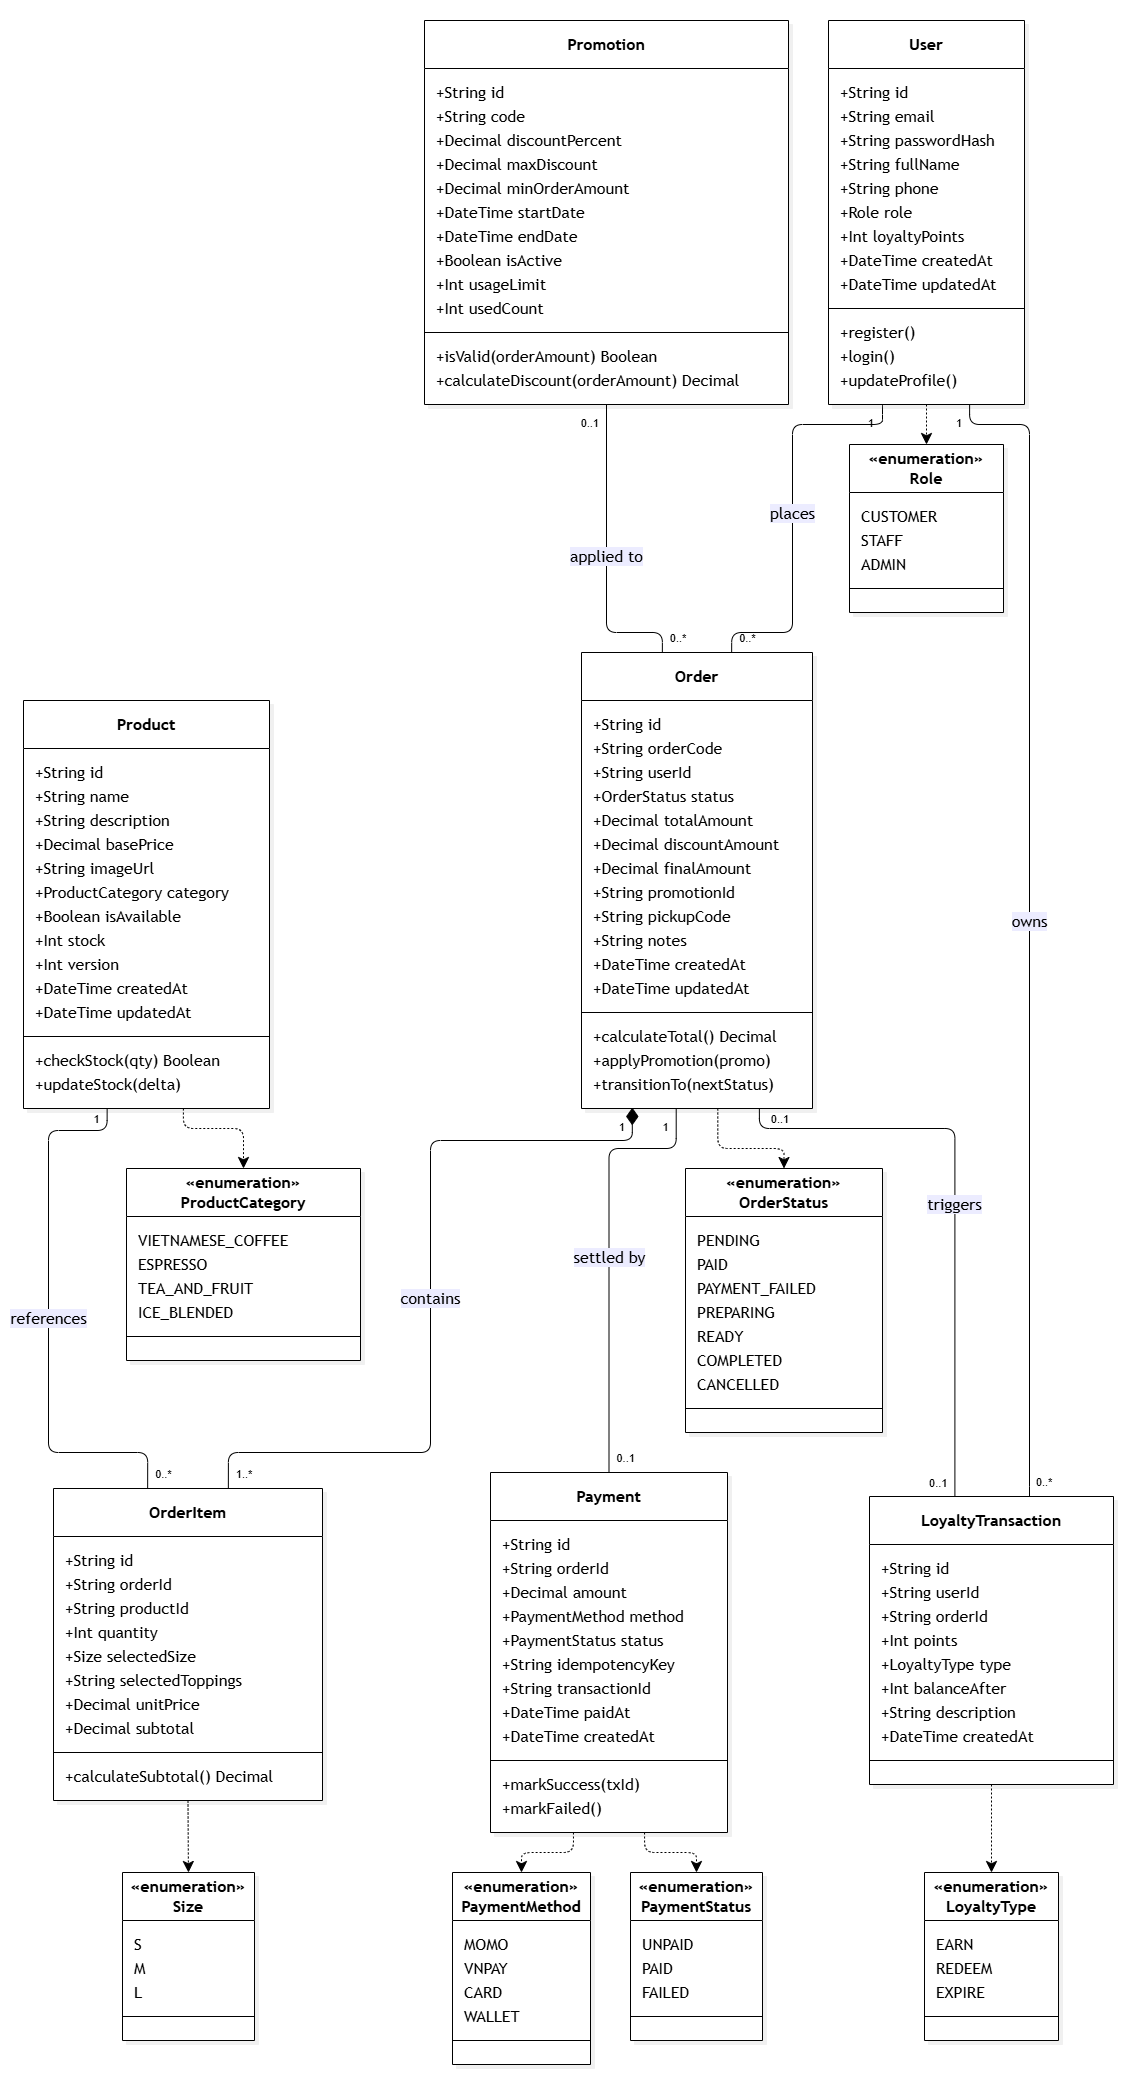
\includegraphics[width=0.85\textwidth,height=0.48\textheight,keepaspectratio]{figures/class-domain.png}
  \caption{Sơ đồ lớp miền nghiệp vụ và quan hệ thực thể hệ thống BrewLite}
  \label{fig:a1-class}
\end{figure}

\subsection{Kiểm chứng Definition of Done (DoD)}
Mọi Task trong Product Backlog đều được nghiệm thu chặt chẽ theo 4 tiêu chuẩn DoD của Mục 10 Assignment 1 (chi tiết tại \texttt{docs/sprint/definition-of-done.md}):
\begin{enumerate}[1.]
  \item \textbf{Chạy ổn định \& không lỗi build:} Đạt 100\% \texttt{npm run lint}, \texttt{npm run typecheck}, \texttt{npm run build} và 32 test suites / 143 tests ở cả Frontend và Backend.
  \item \textbf{Quy chuẩn Git \& Clean Code:} Tuân thủ Conventional Commits trên GitHub, tuyệt đối không chứa comment thừa trong mã nguồn TypeScript/TSX (kiểm chứng tự động bằng AST).
  \item \textbf{Validation \& UX:} API kiểm tra chặt chẽ DTO đầu vào (\texttt{class-validator}); UI xử lý đầy đủ Skeleton Loading, Empty State, Error State và giữ giỏ hàng khi gặp lỗi thanh toán.
  \item \textbf{Tài liệu bàn giao:} \texttt{README.md} hướng dẫn đầy đủ cách chạy cục bộ, chạy kiểm thử và khởi chạy 1 lệnh qua \texttt{docker compose up --build -d}.
\end{enumerate}

\newpage
\section{Bàn giao sản phẩm, Sprint Review và Sprint Retrospective}

\subsection{Hồ sơ bàn giao và Môi trường Demo trực tuyến}
\begin{itemize}
  \item \textbf{Kho mã nguồn GitHub (Tag \texttt{v1.0.0}):} \url{https://github.com/nphat-code/swe-project}
  \item \textbf{Bản triển khai trực tuyến trên AWS EC2 (HTTPS):}
    \begin{itemize}
      \item Giao diện Web / PWA: \url{https://nphat-brewlite.duckdns.org}
      \item Backend REST API: \url{https://nphat-brewlite.duckdns.org/api}
      \item Endpoint giám sát sức khỏe: \url{https://nphat-brewlite.duckdns.org/health} (\texttt{status: ok}, \texttt{db: up}, \texttt{1ms})
    \end{itemize}
  \item \textbf{Chạy cục bộ bằng Docker Compose:} 1 lệnh duy nhất \texttt{docker compose up --build -d} khởi chạy trọn bộ 3 services (\texttt{postgres}, \texttt{backend}, \texttt{frontend}) kèm auto-migration và nạp dữ liệu mẫu.
  \item \textbf{Tài khoản mẫu phục vụ Demo:} Khách hàng \texttt{customer@brewlite.vn} / Barista \texttt{barista@brewlite.vn} (mật khẩu: \texttt{BrewLite@2026}); mã Voucher mẫu: \texttt{BREWLITEFIRST}, \texttt{COFFEELOVER}.
\end{itemize}

\subsection{Sprint Review (Nghiệm thu luồng End-to-End)}
Buổi nghiệm thu cuối Sprint 2 xác nhận vượt qua 8/8 kịch bản trình diễn thực tế:
\begin{enumerate}[1.]
  \item Mở trang Menu, lọc qua 4 danh mục thực tế, tìm kiếm sản phẩm và kiểm tra trạng thái Skeleton/Empty/Error.
  \item Chọn món $\rightarrow$ chọn Size (S/M/L), đa Topping, nhập ghi chú $\rightarrow$ kiểm tra giá tự động cập nhật và thêm vào giỏ hàng Zustand.
  \item Mở \texttt{CartDrawer}, tăng/giảm số lượng, áp mã khuyến mãi \texttt{BREWLITEFIRST}.
  \item Đăng ký tài khoản mới hoặc đăng nhập \texttt{customer@brewlite.vn} nhận JWT Bearer token.
  \item Mở \texttt{CheckoutModal} $\rightarrow$ thử kịch bản thanh toán thất bại (\texttt{PAYMENT\_FAILED}): xác nhận giỏ hàng vẫn được giữ nguyên $\rightarrow$ thanh toán lại thành công chuyển sang \texttt{PAID}.
  \item Kiểm tra màn hình \texttt{OrderConfirmationModal} (mã đơn \texttt{\#xxxxxx}, trạng thái \texttt{PAID}, điểm thưởng Loyalty) và xem lại trong \texttt{OrderHistoryModal} (\texttt{GET /orders/me}).
  \item Chạy bộ kiểm thử tự động chứng minh 3 tiêu chí Task 10 \texttt{(a)(b)(c)} và bộ Supertest HTTP E2E.
  \item Kiểm tra khởi chạy cụm 3 container Docker Compose và truy cập trực tiếp bản Production HTTPS trên AWS EC2.
\end{enumerate}

\subsection{Sprint Retrospective và Backlog phiên bản tiếp theo}
\begin{itemize}
  \item \textbf{Điều làm tốt (What went well):} Hoàn thành đúng 100\% cam kết (23/23 SP Sprint 1, 33/33 SP Sprint 2); tách rõ trách nhiệm giữa Frontend/Backend; giải quyết triệt để các bài toán khó về đồng thời (Idempotency, Optimistic Locking, State Machine) có kiểm thử chứng minh rõ ràng.
  \item \textbf{Điều cần cải thiện (Challenges \& Lessons Learned):} Quản lý chặt đường dẫn build NestJS (\texttt{dist/src/main.js}), cấu hình Next.js Standalone trong Docker (\texttt{DOCKER\_BUILD=true}) và bổ sung cờ \texttt{SEED\_IF\_EMPTY=true} để bảo toàn dữ liệu khi container khởi động lại.
  \item \textbf{Backlog phiên bản v1.1 (Nhận phản hồi khách hàng):} Xây dựng màn hình Kitchen Display System (KDS) thời gian thực cho quầy Barista qua WebSocket/SSE, bổ sung đổi điểm thưởng Loyalty trực tiếp thành mã giảm giá và tích hợp thanh toán QR động thực tế.
\end{itemize}

\newpage
\begin{thebibliography}{80}

\bibitem{scrumguide}
Ken Schwaber, Jeff Sutherland,
\textit{The Scrum Guide -- The Definitive Guide to Scrum: The Rules of the Game},
2020.

\bibitem{sommerville}
Ian Sommerville,
\textit{Software Engineering (10th Edition)},
Pearson, 2015.

\bibitem{nextjs}
Vercel,
\textit{Next.js Documentation -- App Router, React Server Components and Standalone Output},
\url{https://nextjs.org/docs}, 2026.

\bibitem{nestjs}
Kamil Myśliwiec,
\textit{NestJS Framework Official Documentation},
\url{https://docs.nestjs.com}, 2026.

\bibitem{prisma}
Prisma Data, Inc.,
\textit{Prisma ORM -- Transactions, Optimistic Concurrency Control and Migrations},
\url{https://www.prisma.io/docs}, 2026.

\end{thebibliography}

\end{document}

